\section{Code Structure and Simulated Data}
To implement the linear-Gaussian binary latent feature model~\cite{griffiths2005infinite, ibp2012matlab} with IBP as the prior, a Gibbs sampler is used to generate the posterior samples, and the graphical model is shown in Figure~\ref{fig:IBPgeneration}. The IBP function is described in Section~\ref{sub:IBPalg}, and denoted as $Z \sim \text{IBP}(\alpha)$, where $Z$ is the binary matrix and $\alpha \sim Ga(1,1)$.

\begin{figure}
\centering
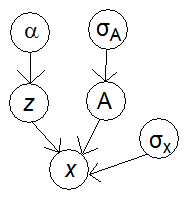
\includegraphics[width=0.25\linewidth]{IBP_generation.png}
\caption {Graphical model for the linear-Gaussian binary latent feature model}
\label{fig:IBPgeneration}
\end{figure}

\subsection{Simulated Data for Likelihood}
\label{sub:simulated}

The likelihood involves simulated image data, and the variables are defined as follows:

\begin{itemize}
\item $N = 100$ is the number of images (customers or objects)
\item $D = 6 \times 6 = 36$ is the length of vectors (dishes or features) for each image
\item $K = 4$ is the number of basis images (latent or underlying variables)
\item $\mathbf{X}$ represents the images generated by the $K$ bases (each basis is present with probability 0.5), with white noises $\text{Normal}(0,\sigma_X^2 = 0.5^2)$ added
\end{itemize}

The likelihood function is
\begin{gather}
\mathbf{X}|(\mathbf{Z},\mathbf{A},\mathbf{\sigma_X}) \sim \text{Normal}(\mathbf{ZA},\Sigma_X = \sigma_X^2\mathbf{I}) \\
P(\mathbf{X} | \mathbf{Z}, \sigma_X, \sigma_A) = \dfrac{1}{(2\pi)^{ND/2} \sigma_X^{(N-K)D} \sigma_A^{KD} |\mathbf{Z}^T\mathbf{Z} + \dfrac{\sigma_X^2}{\sigma_A^2}\mathbf{I}|^{D/2}} \exp\{-\dfrac{1}{2\sigma^2_X} \text{tr}(\mathbf{X}^T(\mathbf{I}-\mathbf{Z}(\mathbf{Z}^T\mathbf{Z}+\dfrac{\sigma_X^2}{\sigma_A^2}\mathbf{I})^{-1}\mathbf{Z}^T)\mathbf{X})\}
\end{gather}

Each object $i$ has a $D$-dimensional vector of properties named $x_i$, where:
\begin{itemize}
\item $x_i \sim \text{Normal}(\mathbf{z_i} \mathbf{A}, \Sigma_X = \sigma_X^2\mathbf{I})$
\item $\mathbf{z_i}$ is a $K$-dimensional binary vector (features)
\item $\mathbf{A}$ is a $K \times D$ matrix of weights, with prior $\mathbf{A} \sim \text{Normal}(0,\sigma_A^2 \mathbf{I})$
\end{itemize}

% Need to generate the images here :)
The four basis images and an example of the simulated data are shown in Figure~\ref{fig:images}. Note that the likelihood involves close-to-zero probabilities, so the log likelihood is used in my code instead.

\begin{figure}[!ht]
\centering
    \begin{minipage}{0.8\linewidth}
    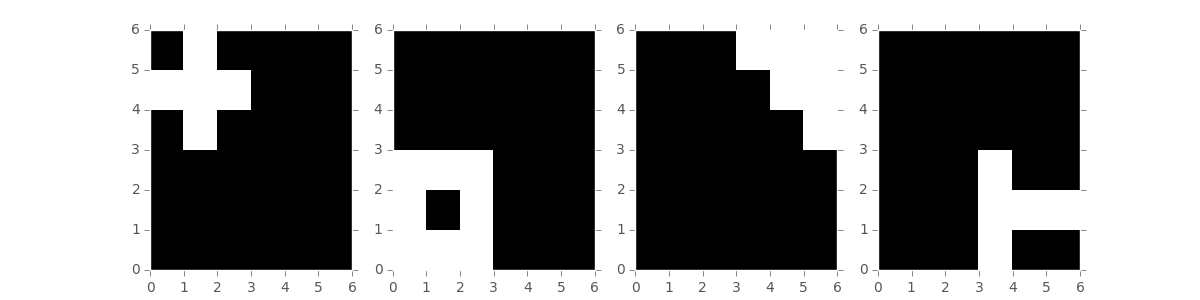
\includegraphics[width=\linewidth]{basis_images.png}
    %\caption{The four basis images}
    %\label{fig:basis}
    \end{minipage}%
    \begin{minipage}{0.2\linewidth}
    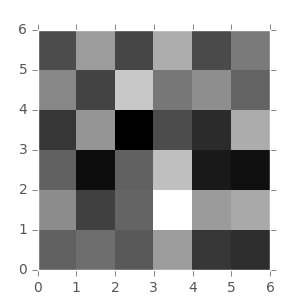
\includegraphics[width=\linewidth]{example_image.png}
    %\caption{An example image}
    %\label{fig:example}
    \end{minipage}
    \caption{Simulated dataset: The four basis images (left) and an example image (right)}
    \label{fig:images}
\end{figure}

\subsection{Gibbs Sampler for the Posterior Distribution}

The full (posterior) conditional distribution is
\begin{equation}
P(z_{ik} | \mathbf{X,Z_{-i,k}},\sigma_X, \sigma_A) \propto P(\mathbf{X} | \mathbf{Z_{-i,k}},\sigma_X, \sigma_A) P(z_{ik} | \mathbf{z_{-i,k}})
\end{equation}

When initializing the Gibbs sampler, set $\sigma_A = 1, \sigma_X = 1, \alpha \sim Ga(1,1)$. Then the sampler does the following steps: ($K$ in my code is denoted as $K_+$, to differentiate it from the true value.)

\begin{enumerate}
\item Generate $P(z_{ik} | \mathbf{X,Z_{-i,k}},\sigma_X, \sigma_A)$ using the full conditional distribution
    \begin{enumerate}
    \item Remove singular features (at most one object has it);\\
    decrease $K_+$ by 1 for each feature removed
    \item Determine each $z_{ik}$ to be $0$ or $1$ by Metropolis
    \item Add new features from $\text{Pois}(\frac{\alpha}{i})$
    \end{enumerate}
\item Sample $\sigma_{X}^* = \sigma_X + \epsilon$, where $\epsilon \sim \text{Unif}(-0.05,0.05)$, and accept $\sigma_{X}^*$ by Metropolis 
\item Sample $\sigma_{A}^* = \sigma_A + \epsilon$, where $\epsilon \sim \text{Unif}(-0.05,0.05)$, and accept $\sigma_{A}^*$ by Metropolis 
\item Generate $\alpha|Z \sim Ga(1+K_+,1+\sum^{N}_{i=1}H_i)$, where $K_+$ is the number of features with $m_k > 0$
\end{enumerate}

The Metropolis part for $\sigma_A$ is demonstrated as follows (similar case for $\sigma_X$):
\begin{itemize}
\item Genenerate a candidate value $\sigma_{A}^{*} = \sigma_{A} + \epsilon$, with $\epsilon \sim \text{Unif}(-0.05,0.05)$
\item Generate a random number $r \sim \text{Unif}(0,1)$
\item Accept $\sigma_{A}^{*}$ if $r < \text{min}\{ 1, \dfrac{P(\sigma_{A}^{*} | \mathbf{Z,X},\sigma_X)}{P(\sigma_{A} | \mathbf{Z,X},\sigma_X)} \}$, where $\sigma_{A}$ is the current value
\end{itemize}

The candidate value $\sigma_{A}^{*}$ is always accepted when the likelihood ratio $\frac{P(\sigma_{A}^{*} | \mathbf{Z,X},\sigma_X)}{P(\sigma_{A} | \mathbf{Z,X},\sigma_X)}$ is larger than 1, i.e. $P(\sigma_{A}^{*} | \mathbf{Z,X},\sigma_X) > P(\sigma_{A} | \mathbf{Z,X},\sigma_X)$. Nevertheless, when the likelihood ratio is less than 1, there is still a non-zero probability to accept $\sigma_{A}^{*}$, so the sampler can ''move forward''. Note that in my code, the log likelihoods are used in the following way:

% including how to normalize the log/relative probabilities
\begin{equation}
\text{min}\{ 1, \dfrac{P(\sigma_{A}^{*} | \mathbf{Z,X},\sigma_X)}{P(\sigma_{A} | \mathbf{Z,X},\sigma_X)} \} = \exp(\text{min}\{0, \log(P(\sigma_{A}^{*} | \mathbf{Z,X},\sigma_X)) - \log(P(\sigma_{A} | \mathbf{Z,X},\sigma_X))\})
\end{equation}

Finally, the posterior expectation of $\mathbf{A}$ is:
\begin{equation}
E(\mathbf{A}|\mathbf{X,Z}) = (\mathbf{Z}^T\mathbf{Z}+\frac{\sigma_X^2}{\sigma_A^2}\mathbf{I})^{-1} \mathbf{Z}^T \mathbf{X}
\end{equation}
This is denoted as $\mathbf{A}_{\text{inf}}$, with size $D \times K_+$, and $\mathbf{A}_{\text{inf}}$ is the matrix of latent features (images) my code converges to.